%vormatierung
\documentclass[12pt,a4paper,bibliography=totocnumbered,listof=totocnumbered]{scrartcl}
%zeilenabstand
\usepackage{setspace}
\onehalfspacing
\parindent 0pt

\usepackage{tabularx}
\usepackage[utf8]{inputenc}
%font änder
\usepackage[ngerman]{babel}
%ränder
\usepackage[paper=a4paper,left=40mm,right=30mm,top=25mm,bottom=25mm]{geometry} 
%Abstand Fusnoten
\deffootnote{1em}{1em}{\textsuperscript{\thefootnotemark\ }}
%sub und subbubsection tiefe
\setcounter{tocdepth}{3}
%Inhaltsverzeignis anklickbar.
\usepackage{hyperref}
\setcounter{secnumdepth}{3}
%sonderzeichen
\usepackage[T1]{fontenc}
%grafiken einbinden
\usepackage{graphicx}
\usepackage{pdflscape}
\usepackage{listings}

\lstdefinestyle{myStyle}{
    backgroundcolor=\color{gray!10},   % Hintergrundfarbe
    basicstyle=\ttfamily\small,        % Schriftart und -größe
    frame=single,                      % Rahmen um den Text
    framesep=5pt,                      % Abstand zwischen Rahmen und Text
    rulecolor=\color{black},           % Rahmenfarbe
    xleftmargin=10pt,                  % Abstand vom linken Rand
    xrightmargin=10pt,                 % Abstand vom rechten Rand
    breaklines=true,                   % Zeilenumbruch zulassen
    breakatwhitespace=true,            % Zeilenumbruch an Leerstellen
    showstringspaces=false,            % Leerzeichen in Strings nicht hervorheben
}


%Wie können künstliche Intelligenzen bei der Entwicklung eines Videospiels in der Unreal Engine 5 eingesetzt werden?
\title{Entwicklung eines Videospielprototypen als ,,Ein-Mann-Videospielentwickler´´ auf der Unreal Engine 5 mit Hilfe von KI-Systemen}

\author{Nicolas Taylor}

\date{11.04.2023}

\begin{document}
\thispagestyle{empty}
\begin{center}
        	
        	\vspace*{1cm}
        	\Large
        	\textbf{Hochschule Fulda}\\
        	\textbf{Fachbereich Angewandte Informatik}\\
        	\vspace*{4cm}
        	
        	\huge
        	\textbf{BA}\\
        	\vspace*{0.5cm}
        	\large
        	
        	\textbf{Entwicklung eines Videospielprototypen als ,,Ein-Mann-Videospielentwickler´´ auf der Unreal Engine 5 mit Hilfe von KI-Systemen}\\
        	\vspace*{1cm}
%    	\includegraphics[scale=1.0]{Bilder/logo.png}\\
%     	\vspace*{2cm}
        	
        	\vfill
        	\normalsize
\newcolumntype{x}[1]{>{\raggedleft\arraybackslash\hspace{0pt}}p{#1}}
        	%\begin{tabular}{x{6cm}p{7.5cm}}
                    	%\rule{0mm}{5ex}\textbf{Autor:} & Nicolas Taylor - nicolas.taylor@gmx.net
                    	%rule{0mm}{5ex}\textbf{Prüfer:} & Prof. Dr. Christian Fischer
                    	%\\
                    	%\rule{0mm}{5ex}\textbf{Abgabedatum:} & 11.04.2023
                    	%\\
        	%\end{tabular}
\end{center}
\pagebreak
\tableofcontents
\newpage
%1
\section{Einleitung}
Sprich mir nach; ich bin Game Designer. Herzlichen Glückwunsch, du bist "Gamedesigner."
\\
Dieses Zitat stammt von Jesse Schell; Hochschullehrer für Unterhaltungstechnologie am Entertainment Technology Center in Pittsburgh, USA.
\\
Wenn er gefragt wird, was er macht, um seine Brötchen zu verdienen, antwortet er: "Ich bin Game Designer". Jesse Schell, ermutigt Anfänger in seinem Buch, die noch vor Ihrem ersten Schritt Game Designer oder Videospiele Entwickler stehen, sich selbst als Gamedesigner zu bezeichnen. Wenn wir den Worten von Jesse Schell Glauben schenken, ist Gamedesigner werden nicht schwer.
\\
Wenn man sich dazu entscheidet Videospiele zu produzieren, steht man am Anfang sehr oft alleine da. Genau um dieses alleine sein, möchte ich mich auf meine Bachelor Thesis beziehen.
\\
Ich benutze in meiner Bachelorthesis den Begriff Ein-Mann-Videospielentwickler, um zu verdeutlichen, dass alle Prozesse an einer Person abhängen.
\\
In der Videospielindustrie ist es heute üblich, dass ein Spiel von Entwickler Studios entwickelt wird, die mehrere hundert Angestellte haben. Zum Beispiel Baldur´s Gate 3 , was von dem Belgischen Entwicklerstudio Larian Studios entwickelt wurde, hat mehr als 450 Angestellte.
\\
Im Jahr 2022 hat ein großes kulturelles Umdenken in unserer Gesellschaft stattgefunden, was das Thema KI betriff. Früher ein Thema für Nerds und Science Fiction, heute ein Thema für Markus Lenz und die Tagesschau.
\\
Bettina Stark-Watzinger bezeichnet KI als Schlüsseltechnologie.
\\
Mein Ziel ist es, als Ein-Mann-Videospielentwickler einen Prototyp im Rahmen meiner Bachelorthesis zu entwickeln mit Hilfe von KI-Systemen.
\\
Genau diese Entwicklung möchte ich in meiner Thesis analysieren und beschreiben.
%https://dailygame.at/baldurs-gate-3-entwickler-bleibt-weiterhin-unabhaengig/ -03.09.2023
 
\subsection{Motivation und Idee}
Videospiele werden aus sehr vielen Teilbereichen der Medienbranche zusammengesetzt, wie zum Beispiel Autoren, Programmierer und Illustratoren bis hin zu Marketing und Vertrieb.
\\
In den Anfangszeiten, wo Videospiele gerade angefangen haben, sich kommerziell als Unterhaltungsmedium zu etablieren, wurde ein großer Teil von Videospielen von einer Person geschrieben. Spiele Wie Space Invader, Adventure oder Space War [arbeitstitel bitte noch mal in der geschichte der VS nachssacuen]
\\
Spätestens in den 90er Jahren wurden nur noch sehr wenige Spiele von einer Person entwickelt die in Arcadehallen oder Kaufhäußer zugänglich waren.
Warum der Ein-Mann-Videospieleentwickler immer seltener wurde, liegt großteil daran, dass die Technik auf denen die Vidoepiele liefen mit der Zeit leistungsfähiger wurden und somit größere und Komplexere Spielewelten erschaffen konnten.
\\
Diese Komplexität der spielewelten konnte nicht mer von einem Einzigen Entwickler gewährleistet werden.
\\
Im Jahr 2022 Hat die Firma OpenAI sein KI-Werkzeug ChatGPT der öffentlichkeit zugänglich gemacht, und viele Berichten von einem Meilenstein in der KI-Forschung.
\\
ChatGPT kann selbständig durch eine für den Menschen einfache Aufforderung Schulaufgaben lösen, oder mit dem Benutzer sich unterhalten.
\\
ChatGPT kann ganze Programme in verschiedenen Programmiersprachen Schreiben, was es davor nie in solchen Umfang dargewesen war.
\\
KI-Systeme bieten ein neues Gebiet um Forschung und Experimente zu betreiben, und ich möchte in meiner Bachelorthesis herausfinden ob es möglich ist, ein Vidospiel, genauer ein Prototyp von einem Videospiel zu entwickel, wie in der Pionierszeit wo einzelne Entwickler ganze Projekte erschaffen.
\\
 
Die Systeme, auf denen Videospiele liefen, wurden immer leistungsfähiger, und somit wurden auch lebendigere und komplexere Welten möglich. Videospiele wurden in der Regel nicht mehr von einer Person entwickelt, sondern von ganzen Studios. In diesen Studios werden Aufgaben auf Teams verteilt, wie zum Beispiel Concept Art and Design, Musik und Soundeffekte bis hin zum Vertrieb und Marketing.
\\
Kurz, ein Videospiel zu entwickeln ist schon sehr lange keine Ein-Mann-Aufgabe mehr, Und in solchen Teams kann jeder Videospielentwickler sich auf seine Stärken im Team konzentrieren.
\\
Ich sehe seit 2022 eine neue Möglichkeit Videospiele zu entwickeln, die zuvor in diesem Umfang nicht möglich gewesen war.
\\
KI-Systeme sind Werkzeuge, die ein hohes Potenzial beinhalten, um schnelles und qualitatives Arbeiten mit sich bringen.
\\
Mit Midjourney kann ich innerhalb von wenigen Minuten eine Landschaft erstellen lassen. ChatGPT kann dir Geschichten schreiben und Voice.ai dir eine neue Stimme verleihen. Das was die vorhin drei genannten KI-Systeme sich spezialisiert haben, sind in der realen
Welt, echte Berufe in der Gamingbranche - Concept Artist, narrative Designer / video game writer, voice actor.
\\
Es ist heute theoretisch möglich, ohne viele Vorkenntnisse diese Aufgaben mit Hilfe von KI-Systemen zu übernehmen.
\subsection{Forschungsfrage}
\subsection{Forschungsmethoden}
Ich werde in dieser Arbeit einen Prototyp entwickeln. Während dieser Arbeit werde ich versuchen, Probleme und Aufgaben mit KI-Systemen zu lösen. Diese Lösungen werde ich in dieser Arbeit präsentieren.
\subsection{Gliederung der Arbeit}%todo hööööö?!
Die Arbeit ist gegliedert in, Warum ich was mache, dann ein Paar allgemeine Erklärungen.
\\
Was ich mache. Und welche Werkzeuge ich benutze. Ich werde Alles am Ende analysieren
\subsection{Zielsetzung}
Mein Ziel in dieser Arbeit ist es, einen Prototyp zu entwickeln. Dieser Prototyp wird nur von einer Peron entwickelt, und alle anderen Aufgaben und Probleme werden versucht, mit Hilfe von KI-Systemen zu lösen.
\subsection{Abgrenzung}
\section{Fragestellung}
KI ist ein großes Technologiefeld, was schon seit 15 Jahren daran geforscht wird. Seit ChatGPT 2022 für die breite Öffentlichgkeit geöffnet wurde, ist ein Bewustsein für diese Technologie geschaffen wurden.
\\
Viele gesellschaftliche, und industrielle gebiete sind oder werden in nahe zukunft mit KI-Systemen ihren Alltag finden.
\\
Viele KI-Systeme können mittlerweile sehr kreative Aufgaben sehr schnell bearbeiten und Resultate hervorbringen.
\\
Bilder, Stimmen, Animationen, Text. Alles Medienformen die in Videospiele benötigt werden um ein Fertiges Produkt zu erzeugen.
\\
Wie weit kommt Stand Heute ein Ein-Mann-Videospieleentwickler, wenn er sich dieser KI-Systeme bedient? Was sind die Hürden? Was sind die Vorteile? Ist es sinnvoll, auf solche Systeme zurückzugreifen, um einen Prototypen zu entwickeln.
\\
Diese Fragen möchte ich in meiner Bachelorthesis klären.
\\
Ich werde selber forschen, welche KI-Systeme es gibt und welche ich wie und in welcher Weise ich benutzen kann, um ein Prototypen zu entwickeln.
 
\section{Theoretischer Hintergrund}
%\\\\\\\\\\\\\\\\\\\\\\\\\\\\\\\\
\subsection{Begriffsdefinitionen}%erläuterung
%\\\\\\\\\\\\\\\\\\\\\\\\\\\\\
\subsubsection{KI-System}
%https://www.bsi.bund.de/DE/Themen/Verbraucherinnen-und-Verbraucher/Informationen-und-Empfehlungen/Technologien_sicher_gestalten/Kuenstliche-Intelligenz/kuenstliche-intelligenz_node.html
Mittels maschinellen Lernens großer Datenmengen, können KI-Systeme, selbständige Lösungskompetenzen erwerben. KI-Systeme können die Fähigkeit besitzen, Eingabedaten, die nicht zu ihren Trainingsdaten vorkommen, zu verarbeiten.
\subsubsection{Prompt}
%https://dict.leo.org/englisch-deutsch/prompts ; https://bm-experts.de/definitionenfaq/definitionen/prompt-was-ist-das-und-wie-kann-er-eingesetzt-werden/
Aus dem Englischen, to prompt, und bedeutet so viel wie auordern oder ab fragen. Der User benutzt Prompts, um einem KI-System einen Befehl zu überreichen. Im Beispiel von ChatGPT gibt der User ein Prompt in das Chatfenster, undb ChatGPT generiert eine passende Antwort.
\subsubsection{NPC}
% (DKDG) Klaus Breuer - Computerspiele programmieren - Künstliche Intelligenz für Künstliche Gehirne - Kapitel 15.1 Erster Absatz Seite 113 ------ Computerspiele programmieren: künstliche Intelligenz für künstliche Gehirne / Breuer, Klaus Barcode 12155751 Rückgabe bis 12.06.2023
Non-Player Characters, kurz NPC, sind vom Computer gesteuerte Charaktere, Dorfbewohner, Tiere oder Monster. Alle Charaktere und Tiere, die sich nicht vom Spieler kontrollieren lassen. NPCs sind notwendig, um eine Spielwelt lebendig wirken zu lassen.
\subsubsection{Game Designer}
%Die Kunst des Game Designs : bessere Games konzipieren und entwickeln / Schell, Jesse Barcode 12486880 Kapitel 1.2 Seite 35 bis 37 DKDG
Ein Game Designer besitzt ein breites Spektrum an Fähigkeiten wie Animation, Architektur, Betriebswirtschaft, Game Engineering, Darstellende Kunst, Geschichte, Management, Mathematik, Musik, Präsentation, Soundgestaltung, Spiele und viele weitere beherrschen sollte.
\\
Der Game Designer erschafft ein Erlebnis, wobei das Spiel nicht das Erlebnis ist, sondern nur die Möglichkeit, dem Spieler ein Erlebnis zu erleben.
%Kapitel 2.1 Seite 44
\subsubsection{Design}%Seite 49 oder eine andere gemeingültige Quelle DKDG
\subsubsection{Spiel}%Kapitel 4.2 seite 74 bis 89-- Großes Kapitel
\subsection{Videospiel-Entwicklung}
\subsubsection{Die Vier Grundelemente eines Videospiels}%Kapitel5.2 Seite 93 DKDG
\subsection{Unreal Engine 5}
%https://www.unrealengine.com/de/unreal-engine-5 abrufdatum 27.05.2023
Die Unreal Engine ermöglicht den Spieleentwickler 3D-Videospiele zu entwickeln. Die Entwicklung eines Videospiels in der Unreal Engine 5 kann in Echtzeit entwickelt werden, das bedeutet, dass man das Ergebnis seiner Arbeit sofort betrachten kann. Epic Games, die Entwickler der Unreal Engine 5, beschreiben sie als "Das weltweit offenste und fortschrittlichste Tool zur 3D-Erstellung in Echtzeit".
\subsubsection{Narnite}
\subsubsection{Lumen}
\subsection{Künstliche Intelligenz und ihre Anwendungen in der Videospiel-Entwicklung}
\subsection{Vor- und Nachteile des Einsatzes von KI in der Videospiel-Entwicklung}
%3
\section{Methodik}
\subsection{Auswahl und Beschreibung der KIs}
\subsubsection{ChatGPT}
\subsubsection{Midjourney}
\subsubsection{PIFuHD}
\subsubsection{Voice.AI}
\subsubsection{Adobe Enhanced Speech}
\subsection{Beschreibung der Tools und Technologien}
\subsubsection{Blender}
\subsubsection{Audacity}
\subsection{Beschreibung des Entwicklungsprozesses}
%4
\section{Umsetzung}
\subsection {Idee und Konzeption}
Meine Idee ist ein Videospiel zu entwickeln, das eine geschichtliche und kulturelle Relevanz zur deutschen Geschichte hat. Ein weiteres Kriterium an meinem Videospiel ist es, ein Szenario zu wählen, das sich vor dem Zweiten Weltkrieg befindet. Mit dieser Idee ging ich zu ChatGPT und habe folgenden Prompt formuliert und anschließend diese Ausgabe bekommen.
\begin{figure}[h]
        	\centering
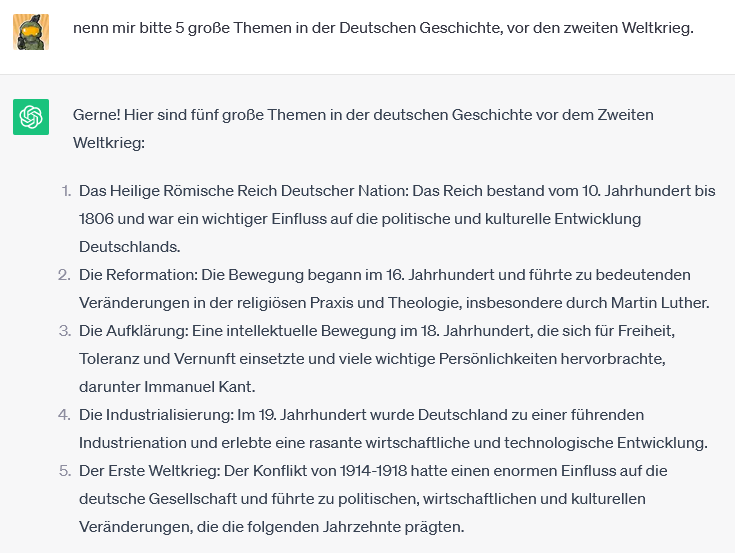
\includegraphics[scale=0.7]{BilderFuerBA/CGPTBachelorarbeitZurKI/01.png}
        	\caption{Ersten 5 Themen}
        	\label{fig:ersten-5-themen}
\end{figure}
\begin{figure}[h]
        	\centering
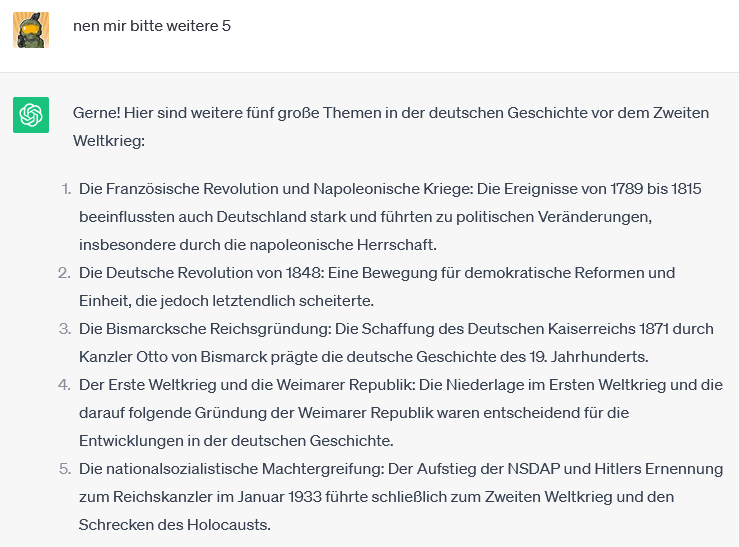
\includegraphics[scale=0.7]{BilderFuerBA/CGPTBachelorarbeitZurKI/02.png}
        	\caption{Zweiten 5 Themen}
        	\label{fig:zweiten-5-themen}
\end{figure}
Man kann an diesem Beispiel sehen, dass ChatGPT mir 10 Ideen präsentiert, die ich in meinem Videospiel verarbeiten kann.
\\
Als Ein-Mann-Videospielentwickler entschied ich mich für die Reformation mit Martin Luther als Hauptfigur.
\\
Innerhalb dieser Bachelorthesis ist es mir aus Zeitgründen nicht möglich ein komplettes Videospiel zu entwickeln, was das Leben von Martin Luther widerspiegelt. Durch meine Recherche über Martin Luther und sein Leben fand ich den Moment bedeutend wo Martin Luther seine 96 Thesen an das Kirchtor nagelt.
\\
In meinem Prototyp werde ich dieses Ereignis als Thematischen Mittelpunkt wählen.
\\
Meine Spielidee für meinen Prototyp ist nun, dass Martin Luther durch ein Dorf läuft, verschiedene NPCs trifft und mit ihnen in einen Dialog tritt. Martin Luther trifft verschiedene Personen mit verschiedenen Problemen und Ansichten. Er redet mit ihnen und lässt sich von ihnen inspirieren. Durch diese Inspiration entwickelte Martin Luther später im Spiel, seine 96 Thesen.
\\
Kern des Prototyps ist die Entwicklung einer Spielwert, die aus einem Dorf mit verschiedenen Häusern und NPCs besteht.
\\
Die Entwicklung des Prototyps unterteilt sich in verschiedene Meilensteine:
-Hauptfigur
\\
-Landschaft
\\
-Gebäude
\\
-Nebenfiguren
\\
-Dialogsystem
\\
-Sprachausgabe
\\
Jeder dieser Meilensteine besitzt in dieser Theses sein eigenes Kapitel, in dem die Entwicklung nahegebracht wird.
\subsection {Meilenstein: Hauptfigur}
\begin{figure}[h]
        	\centering
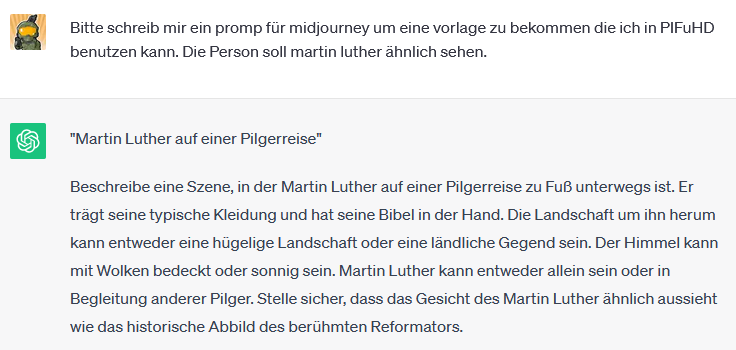
\includegraphics[scale=0.7]{BilderFuerBA/CGPTMidJourneyMartinLuther/01.png}
        	\caption{Erster Versuch: ChatGPT erstellt Promt für Midjourney}
        	\label{fig:chatgpt-ptompt-Midjourney-01}
\end{figure}
\begin{figure}[h]
        	\centering
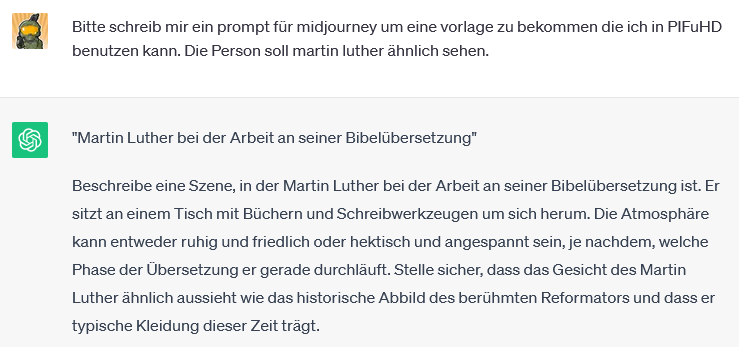
\includegraphics[scale=0.7]{BilderFuerBA/CGPTMidJourneyMartinLuther/02.png}
        	\caption{Zweiter Versuch: ChatGPT erstellt Promt für Midjourney ohne Rechtschreibfehler}
        	\label{fig:chatgpt-ptompt-Midjourney-02}
\end{figure}
\begin{figure}[h]
        	\centering
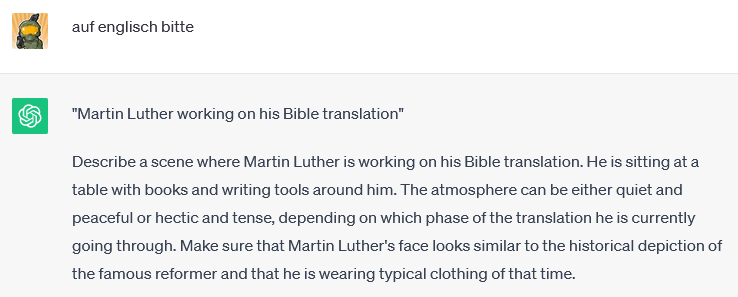
\includegraphics[scale=0.7]{BilderFuerBA/CGPTMidJourneyMartinLuther/03.png}
        	\caption{Dritter Versuch: ChatGPT erstellt Promt für Midjourney in Englisch}
        	\label{fig:chatgpt-ptompt-Midjourney-03}
\end{figure}
Der erste Versuch hat einen deutschen Prompt ausgegeben, der anschließend übersetzt wurde.
\\
Dieser Prompt wurde Midjourney übergeben, was diese Bilder als Resultat ergibt.
[BILD]
ChatGPT beschrieb sehr atmosphärisch, was in ein sehr unaufgeräumtes Resultat hervorbringt.
Es wird vermutet, dass ChatGPT nicht genügend darauf trainiert ist, wie Midjourney Prompts auszusehen sind.
\\
Eine Recherche auf YouTube hat gezeigt, dass das Verwenden von Midjourney-Formeln ein aufgeräumtes Ergebnis hervorrufen kann. Diese Formel wurde ChatGPT übergeben und diese hat ein Aufgeräumteres Ergebnis die Folge.
\begin{figure}[h]
        	\centering
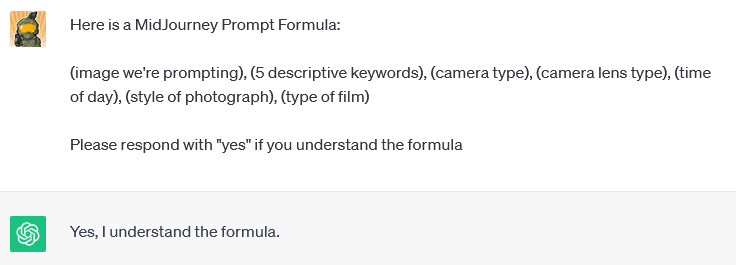
\includegraphics[scale=0.7]{BilderFuerBA/CGPTMidJourneyMartinLuther/04.png}
        	\caption{Vierter Versuch: Aufforderung ChatGPT verwendung einer Midjourney-Formel}
        	\label{fig:chatgpt-ptompt-Midjourney-04}
\end{figure}
\begin{figure}[h]
        	\centering
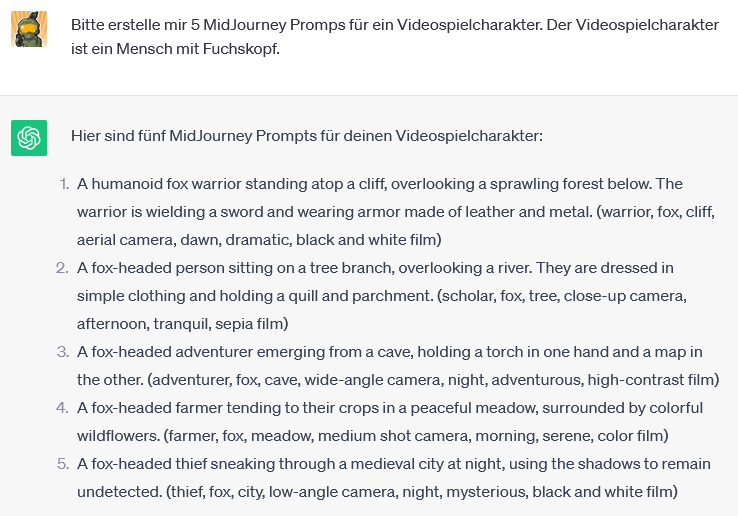
\includegraphics[scale=0.7]{BilderFuerBA/CGPTMidJourneyMartinLuther/05.png}
        	\caption{Erster Test MJ-Formel: ChatGPT erstellt Promt mit verwendung der Midjourney-Formel}
        	\label{fig:chatgpt-ptompt-Midjourney-05}
\end{figure}
\begin{figure}[h]
        	\centering
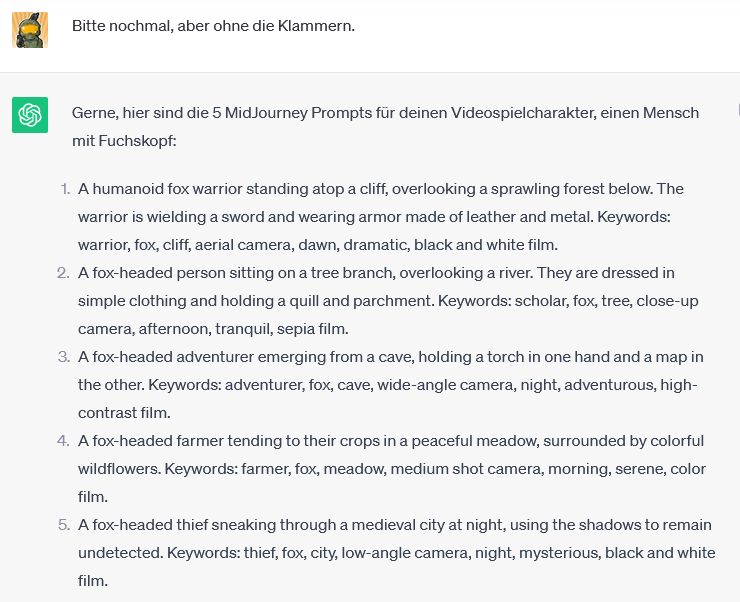
\includegraphics[scale=0.7]{BilderFuerBA/CGPTMidJourneyMartinLuther/06.png}
        	\caption{Zweiter Test MJ-Formel: ChatGPT erstellt Promt für Midjourney in Englisch ohne Klammern}
        	\label{fig:chatgpt-ptompt-Midjourney-06}
\end{figure}
Im ersten Test werden die Prompts mit Klammern ausgegeben. Diese sind mit einer einfachen Aufforderung möglich zu entfernen.
\\
Mein ziel ist es Bilder von Midjourney zu erhalten, die wie Fostos von Personen wirken. Mit diesen Fotos dienen dazu mit PIFuHD zu übergebn um 3D-Modelle von einer Person zu bekommen.
\\
Dieses Modell möchte ich in meinem Prototyp verwenden um eine Spielfigur zu erzeugen.
\\
Ich habe den Promt von ChatGPT so verwendet damit ich ein sauberes Ergebnis bekomme, damit die Vorraussetzun.
\\
PIFuHD weist darauf hin, dass ein neutraler Hintergrund und eine frontalaufnahme die besten vorraussetzung für die verarbeitung eines Bildes zu einem ED-Modell.
\\
Nachdem ich ein Ergebnis von Midjourney erhalten habe, die Martin Luther nachempfunden ist, gebe ich das bild PIFuHD um ein 3D-Modell zu erhalten.
\\
PIFuHD lauffährig zu machen sind einige Einstellung nötig, diese werde ich im Folgenden Kapitel erläutern
 
Über Google Collab ist es möglich PIFuHD zum laufen zu bringen in dem man eine Versionn in sein Google-Drive coopiert.
\\
Über Verbinden und Local Host läuft PIFuHD auf meinem Computer.
\\
 
 
 
 
%[BILD]
%[BILD]
\subsection {Meilenstein: Gebäude}
\begin{figure}[h]
        	\centering
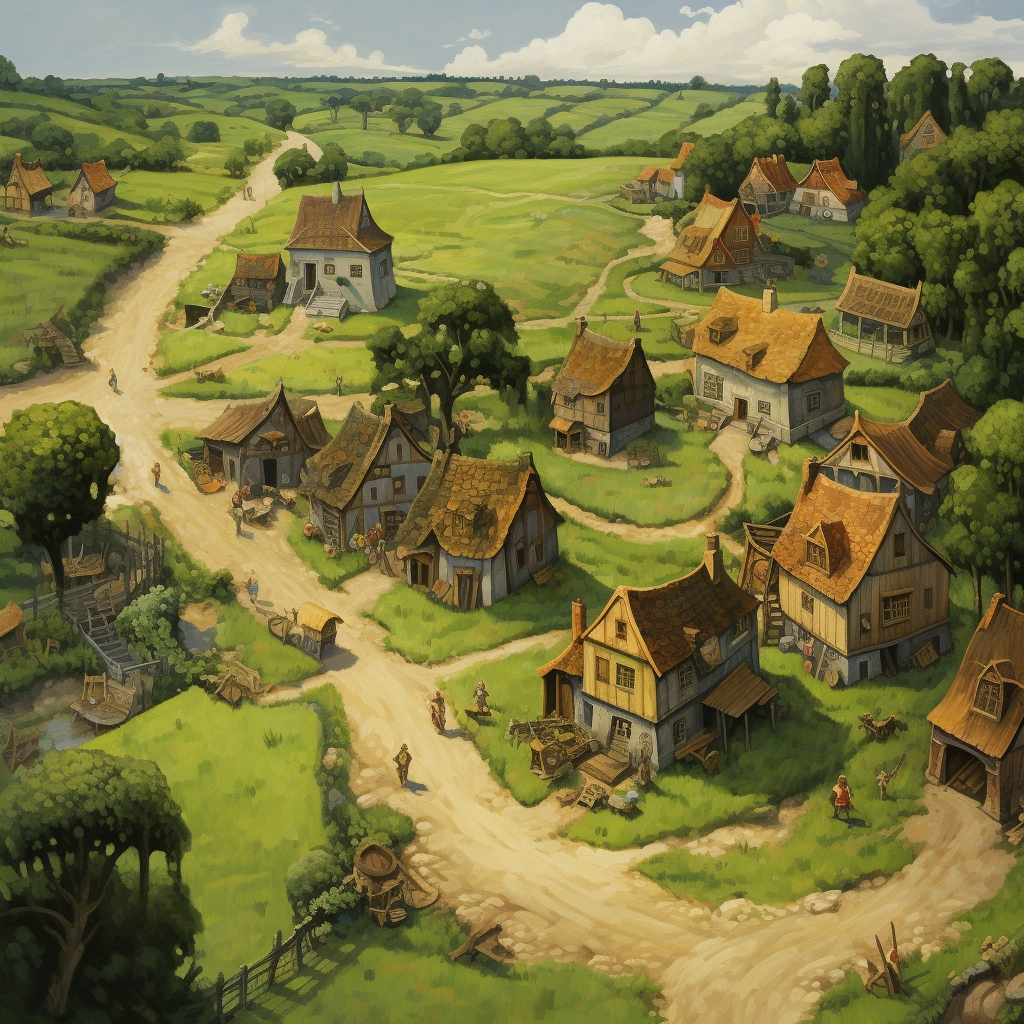
\includegraphics[scale=0.2]{BilderFuerBA/MeilensteinGebaude/a_scatch_from_a_village_top_down.png}
        	\caption{a scatch from a village, top down}
        	\label{fig:Midjourney-Conceptart-Dorf}
\end{figure}
Nach der Erstellung der Hauptspielfigur, ist der nächste Schritt das Erstellen einer Spielwelt.
\\
Die Idee ist es, ein Dorf in der Unreal Engine 5 zu erschaffen. In diesem Dorf befinden sich verschiedene Gebäude.
\\
In diesem Kapitel möchte ich zeigen, wie ich die Gebäude mit Hilfe verschiedener KI-Systeme in der Unreal Engine 5 realisiert habe. Ich werde in diesem Kapitel und in den folgenden Meilensteine nicht mehr so detailliert alles wie bei der Erstellung der Hauptfigur, sondern nur auf Schritte eingehen, die im Prozess unterscheiden.
\\
Fachwerkhäuser repräsentieren etwas Mittelalterliches, und da die Renaissance an das Mittelalter zeitlich gegliedert ist, waren in Zeiten der Renaissance Fachwerkhäuser sehr weit verbreitet.
\\
Meine Idee ist es, Diverse Fachwerkhäuser zu erschaffen und auf einer Landschaft zu verteilen, um eine Dorflandschaft zu kreieren.
\\
Mein erster Ansatz ist es, Häuser mit Hilfe von einem einfachen 3D-Modell umzusetzen, was ich in Blender erstellt habe. Dieses 3D-Modell bestand aus einem Quader mit einer Spitze. Kurz, ein einfaches Haus.
\\
Mit Midjourney habe ich Texturen erstellt, die Fachwerkhäuser nachempfunden sind. Diese Texturen und das einfache Haus wurden mit Hilfe von Blender verbunden. 
\\
Folgend wurden die einfachen Fachwerkhäuser in Unreal Engine 5 Importiert und verteilt.
\\
Die erste Ansatz funktioniert, bringt aber ein Problem mit sich - die Modelle wirken etwas platt und langweilig. 
\\
Besonders da die Kamera sich direkt hinter der Spielfigur befindet und frei schwenkbar ist. Anders, wenn die Kamera so angeordnet ist, wenn sie nur von oben herab schaut. Dafür wären solche Modelle wiederum sehr gut geeignet.
\\
Dieser Ansatz ist nicht gut geeignet, denn die Hauptfigur bewegt sich in der Third-Person durch die Spielwelt. Das Problem mit der Third Person ist, dass man Objekte sehr nah betrachten kann und dadurch unschöne Modelle eher  negativ auffallen als zum Beispiel in der Top-Down-Perspektive, wo 3D-Modelle nur von oben zu betrachten sind.
\\
Eine Inspiration für meinen zweiten Ansatz ist Valheim, ein Survival-Spiel von den Coffee Stain Studios. In diesem Spiel gibt es ein Baukastensystem, in dem der Spieler sein eigenes Haus bauen kann.
\\
In Valheim kann der Spieler verschiedene Wände, Balken, Fußböden, Dächer und Materialarten auswählen, um damit seine Behausung zu gestalten.
\\
Hinzu kommen andere Elemente wie Zäune und Gemüse um ein Garten zu erschaffen, Werkbänke, Tische und Stühle um eine Inneneinrichtung zu kreieren und sogar Teppiche aus Tierfelle und Trophäen die man an die Wand hängen kann um eine Dekorative charakter in die Behausung eines Spielers zu schaffen.
\\
Aus dieser Inspiration habe ich einen zweiten Ansatz entwickelt und zwar einen so genannter Dorfbaukasten.
\\
Dieser Dorfbaukasten besteht ebenfalls aus Wänden, Balken, Dächer, Fußböden und Tapeten.
\\
Im Grunde genommen besteht ein Fachwerkhaus auch aus simplen Bauteilen, wie zum Beispiel Wände, Balken, ein Dach, Türen und Fenster. Diese einzelnen Elemente möchte ich nachbauen, so dass man im Unreal Engine Editor ein Haus selber bauen kann.
\\
Ziel ist es, diese einzelnen Elemente zu programmieren, damit die Materialeigenschaft sich untereinander unterscheiden. Zum Beispiel wirkt jeder Balken unterschiedlich, weil durch Midjourney fünf unterschiedliche Holzmaterialien erstellt wurden.
\\
Mein erster Ansatz war gut, aber nicht gut genug. Ich habe mich als ein Mann Videospiel Entwicklung gegen meinen ersten Ansatz entschieden. Nach der Implementierung in der Unreal Engine 5, sahen die 3D-Modelle für mein Geschmack etwas zu plastisch und platt aus. Die Balken innerhalb. Des Fachwerks haben keine Schatten geworfen und.  Sah einfach zu künstlich aus für meinen Geschmack. Also habe ich einen zweiten Ansatz entwickelt. Der zweite Ansatz besteht aus einem Baukastensystem, jeder Balken, jede Wand und jedes Dachelement hat.  Eine eigenes Element.  Diese Elemente können kann ich die diese Elemente, die in der Regel aus. Einfachen Formen wie?
 
Quader, oder? Dreiecke bestehen.  Kann ich einfach mit einem blueprint Skript.  Die Texturen jeweils. Hinzufügen.  Das bedeutet, ich brauche keinen Blender mehr, um ein 3 D Modell zu erzeugen, sondern mit einfachen.  Formen. Geometrien. Die über die andere Engine.   Mir zur Verfügung gestellt werden.  Mir einen einfachen Bausatz erstellen kann, die ich dann zusammengesteckt. Zusammenstecken kann. Um halt einfache Fachwerkhäuser. Zu erstellen.  Der Vorteil meines zweiten Ansatzes liegt darin, dass ich. Individuellere. Gebäude erstellen kann.
 
Die Sicherheit. Klar, auch in Form.  Von den Nachbarnhäusern unterscheiden.  	Ein weiterer Vorteil ist, ich kann Innenräumen gestalten, das in der ersten Version nicht. Möglich gewesen ist. Oder möglich ist.    	Ich kann mit der zweiten Version Innenräumen auch Fußboden gestalten. Ich kann Tapeten gestalten.
 
\subsection {Meilenstein: Nebenfiguren}
Beim dritten Meilenstein Nebenfiguren möchte ich gerne beschreiben, wie ich meine Nebenfiguren, kurz NPCs, erstellt habe. Ähnlich wie beim Erstellen der Hauptfigur habe ich durch Chat GPT mir verschiedene NPCs beschrieben lassen. Zu dieser Beschreibung gehörte Alter, Geschlecht, Beruf unnd charakterliche Eigenschaften.
\\
Mit diesen Beschreibungen habe ich mir einen Prompt mit hilfe der Midjourney-Formel überlegt und Midjourney hat mir Conceptgraphiken erzeugt. Nach mehreren Versuchen habe ich zwei Conzeptgraphiken bekommen die ich für PIFuHD verwenden kann.
\\
Nach dem ich PIFuHD die beiden Conzeptgraphiken übergeben habe, wu rden sie Wie bei der Hauptfigur in Blender der Polycount reduziert und Texturiert.  Stark verformete stellen die an den Händen und Füßen auftreten wurden im Eddit Mode, oder im Sculp Mode nachgebessert.
\\
Für den Prototyp impotiere ich die NPCs ohne Sceleton Mesh ein, da sie keine Laufanimation benötigen, sonder nur in der Spielwelt plaziert werden um mit dem Hauptcharakter zu reden.
\\
Dadurch das die NPC keine Sceleton Mesh besitzen ist auch gut zu erkennen, das die NPCs keine großen verformungen aufweisen wie die Hauptfigur. Die Verformung tritt z. B. in bereich der Hüfte sehr stark auf aufgrund der unterschiedlich gewichtete zuweisung der Vertices zu den einzelen Bones des Sceleton Mesh.
 
\subsection {Meilenstein: Dialogsystem}
Um ein Dialogsystem in der Unreal Enginge 5 zu entwickeln habe ich mehrere Ansätze gebraucht.
 
Ansatz 1 mit ChatGPT
Ich habe ChatGPT dazu Aufgefordert mir ein Dialogsystem zu entwickeln damit mein Hauptcharakter mit den NPCs aus meinem Prototyp sich unterhalten können.
 
Ich habe versucht die Schritte umzusätzen die ChatGPT mir vorgegeben hat – Erfolglos.
 
Ansatz 2 Rechersche mit Suchmaschienen im Internet
Mit der Suchmaschiene Google
Durch Google bin ich auf ein Video auf Youtube gestoßen, was mir erklärt hat wie ich ein Dialogsystem in Unreal Engine 5 erstellt wird.
\\
Zu dem beschreibenen Dialogsystem wurde von mir noch ein Dilay in der Länge von dem Soundfile hinzugefügt und ein Bool, der auf false steht, falls eine Interaktion gerade nicht möglich ist, zu beispiel ein Charakter redet gerade noch. Dieser Bool soll verhindern, damit keine Dialoge schnell hintereinander gestartet werden und die Charaktere aussprechen lässt.
\\ 
Um die Sprachausgabe zu managen, braucht es ein Dialogsystem. Für das Dialogsystem habe ich
versucht, eine art Dialog System zu erschaffen, das man zum Beispiel aus der Sincefiction Spielereihe Mass Effect kennt. In dem der Spieler verschiedene Antworten- oder Fragemöglichkeiten besitzt. Das hat leider nicht von seiten ChatGPT nicht geklappt.
\\
Ich habe auch ChatGPT gefragt, wie ich ein Dialogsystem in der Unreal Engine 5 umsetzen kann. Auch das hat leider nicht funktioniert. 
\\
An dieser Stelle ist gut zu erkennen das KI-Tool sehr gute ergebnisse erzeugen kann um ein Videospielprototypen zu entwickeln, aber KI-Systeme haben ihre Grenzen, sowie ich Als Ein-Mann-Videospiele-Entwickler auch grenzen habe in der Kompetenz diese Systeme zu bedienen.
\\
Das Problem, dass ich nicht weiß wie ein Dialogsystem entwickelt wurde, und ChatGPT mir ein Falsche lösung mir überreicht hat, habe ich durch die Suchmaschiene von Google und Youtube ein Tutorial gefunden wie ich ein Dialogsystem zwischen meiner Hauptfigur und den NPCs entwickeln kann.
\\
Also habe ich gegoogelt und auf youtube ein Tutorial gefunden.   	Mit der andere Engine 5. Musste ich eine Schnittstelle, was zwischen den verschiedenen.  Actors wie zum Beispiel der Hauptfigur und den MPC.  Eine Schnittstelle bildet.         	Diese Schnittstelle habe ich mit Blueprince umgesetzt. Ich musste auch bei blueprint m bei meiner Hauptfigur Martin Luther.   	Etwas entwickeln und zwar habe ich ein Array erzeugt oder mehrere Arrays erzeugt. Die speichert, was gesagt wird, in Schriftform und was gesagt wird in.   Ausgabe.  In Sprachausgabe, in Soundausgabe.
\\
Ich habe eine Aktionsbutton hinzugefügt, was für was in diesem Beispiel der Buchstabe auf der Tastatur e ist.  Der sagt, Hey, ich möchte mit dir arbeiten.     	Ich habe einen Pool A erzeugt, die. Signalisiert. Hey, ich kann jetzt interagieren mit der Person oder gerade nicht.        	Da das Dialogsystem. Vor z GPT unvollständig war habe ich mir noch andere Dialog Dialoge hinzu ausgedacht, andere Dialoge ausgedacht.  Und somit war das Dialogsystem auch schon fertig.
 
\subsection {Meilenstein: Sprachausgabe}
Nachdem ich das Dialogsystem erstellt und implementiert habe, fehlt nur noch der Inhalt, was die Charaktere miteinander als sich erzählen. Und zwar habe ich hier zwei neue Ki-Systeme benutzt, die vorher noch nicht zum Einsatz gekommen diese sind Voice AI und Adobe Enhance Speache.
\\
Voice AI ist ein KI-System, die Stimmen verändern kann. Zum Beispiel kann man seine Stimme so manipulieren, das sie wie die von Kanye West oder dem amtierende US-Präsident Joe Biden klingt. 
\\
Adobe Enhanced ist ein KI-System, das deine gesprochene Stimme so klingen lässt, dass sie in einem hochwertigen Tonstudio aufgenommen wird.
\\
Meine Sprachaufnahmen verwende ich das Mikrofon von dem Logitech G35 Headset was seit 2014 nahezu täglich benutz wird.
\\
Durch die Kombination von Adobe Enhance Speech und Voice AI habe ich qualitativ hochwertige Sprach Dateien erzeugen können, die sonst ein hochwertiges Tonequipment und gute Dämmung in meinem Büro erzeugt hätten.
\\
Um die Stimmen für die NPCs zu erzeugen, habe ich drei verschiedene Experimente durchgeführt.
\\
\subsubsection{Erst Adobe Enhance Speache dann Voice AI}
Als erstes wurde der Klang meiner stimme mit Audacity und meinem Logitech G35 Headset aufgenommen.
\subsubsection{Erst Voice Ai dann Adobe Enhance Speech}
\subsubsection{Erst Adobe Enhance Speech dann Voice AI dann wieder Adobe Enhance Speech}
 
Experiment eins, erst Voice I gegeben und dann Adobe Anshan Speech.      	Oder? Erst Adobe, Assange Speech und dann Voice AI.  Ich habe noch eine dritte.
\\
Variante ausprobiert, und zwar eine Art Sandwich Methode, indem ich meine Sounddatei, die ich mit Audacity aufgenommen habe, erst Adobe 1. Hand speech. Dann Voice I und dann wieder Adobe A Speech gegeben habe, um so eine Art zweifache Reinigung. Der Sprache oder der Sprachausgabe zu erhalten. 	Mein persönliches bestes Ergebnis, was auch Zeittechnisch am. Sparsamsten war.  Ist erst.  Athan Speech zu benutzen und dann Voice I. Die dritte Version ist auch ok, aber es kann sein, dass danach sich die Stimme noch etwas künstlicher, Blecherner anhört.   Generell ist die Sprachausgabe sehr.  Gut.
\\
Und professionell anwendbar für mein Prototyp ist das eine Qualität, die ich früher nicht erreicht hatte können außer mit großen Aufwand und Kosten verbunden wie ZB das Kaufen eines 200€, Mikrofons und sehr guter Dämmung in meinem Aufnahmeraum. Ich habe die Aufnahmen bei einem sonnigen Tag während. Traktoren im Hintergrund arbeiten. Ich habe in meinem Arbeitszimmer. Ein Fenster aufgehabt. Das offenbar zu einem Bauernhof in meiner Nachbarschaft. Man kann Traktoren hören, man kann meine Frau hören, im Hintergrund, die in der Wohnung mit den Kindern sich beschäftigen und anhand Speech hat das alles herausgefiltert. Und ein gewisses Grundrauschen befindet sich auch nicht mehr und der Sound-Datei.
\\
Die Meilensteine.  Die ich hier in meiner Bachelor thesis beschreibe.  Sind nicht chronologisch sortiert, sondern nur logisch.  Ich habe das Dialogsystem und die Sprachausgabe gleichzeitig entwickelt und.  Implementiert.  Die Sprachausgabe, die ich hiermit mit Voice I und Adobe anhand Speech. Geschaffen habe, habe ich nun in das.  Dialogsystem was sich in dem vorigen Kapitel beschrieben habe. Implementiert. Ich habe die Sprachausgabe in das Array getan.     	In der andere Engine 5.
 
\subsection{Erstellung von Musik und Klängen}
\subsection{Erstellung von Animationen}
\subsection{Entwicklung der Spiellogik}
%5
\section{Ergebnisse und Diskussion}
\subsection{Vorstellung des fertigen Videospiels}
 
\subsection{Diskussion der Ergebnisse und Einschätzung des Erfolgs des KI-Einsatzes}
\subsubsection{Einsatz von MonsterMash}
Monster Mash ist ein KI-System, mit dem man Monster erstellen kann. Wenn man sich realitätsnahe Ergebnisse wünscht, wird man mit Monster Mash auf sehr große Herausforderungen treffen.
\\
Monster sind Fantasiewesen, und niemand kann genau beschreiben, wie ein Monster aussieht. Bei der Darstellung von Menschen oder Gebäuden sieht das anders aus. Für mein Adventure-Game, mit einem historischen Hintergrund, ist MonsterMash nicht zu empfehlen.
\\
Anders würde es in einem Fantasy-Szenario aussehen, wo undefinierte Gestalten dem Spieler begegnen sollen.
\subsubsection{Einsatz von PFuHD}
PIFuHD ist eine KI-System was darauf trainiert ist, Digitalfotos von Personen in ein 3D-Modell umzuwandeln. PIFuHD kann man auf Google-Collab einrichten und lauffähig machen.
\\
Für das erstellen von 3D-Modellen wurde PIFuHD ist in der kostenlosen Demo-Version verwendet.
\\
Die Kompatibilität zwischen Midjourney und PIFuHD ist möglich. Die Resultate sind zum teil Artefakt belastet, die besonders in Bereichen der Hände, Füße und Kleidung auftreten.
\\
Durch Midjourney konnte ich Bilder von Martin Luther erzeugen, die als Konzeptgrafiken dienten. Diese Konzeptgrafiken habe ich PIFuHD als eingabe gegeben, und hat mir daraus folgende 3D-Modelle von Personen ausgegeben, die im Prototyp als Hauptfigur und NPCs verwendet wurden.
\subsection{Kritische Reflexion des Entwicklungsprozesses und Ausblick auf mögliche zukünftige Entwicklungen}
%6
\section{Fazit}
KI-Systeme sind gute Werkzeuge um ein Prototyp
\subsection{Zusammenfassung der Ergebnisse}
\subsection{Implikationen für die Praxis}
\subsection{Limitationen der Studie}
%7
\section{Literaturverzeichnis}
%8
\section{Anhang}
\subsection{Abbildungen und Diagramme}
\subsection{Code-Beispiele}
\subsection{Weitere Materialien}
\end{document}
 
 
%erklärungen wie welche programme eingerichtet und benuttz werden können als Anhang hinzugefügt werden

%hallo test eins



%\subsection{Nutzung von KIs zur Erstellung von 2D Bildern}
%Als erstes brauche ich eine Spielfigur die Martin Luther nachempfunden ist. Mein Worklfow besteht darin ein Promt von ChatGPT ausgeben zu lassen, den ich Später für Midjourney benutzen kann. Genau diesen Prompt habe ich ChatGPT übergeben.
